\begingroup
	\pgfdeclarelayer{background layer}
	\pgfsetlayers{background layer,main}
	\tikzstyle{zero}=[circle,draw=black,fill=white,inner sep=0pt,minimum size=2.5mm]
	\tikzstyle{one}=[circle,draw=black,fill=black,inner sep=0pt,minimum size=2.5mm]
	\tikzstyle{two}=[circle,draw=black,fill=gray,inner sep=0pt,minimum size=2.5mm]
	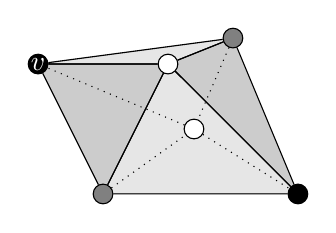
\begin{tikzpicture}[scale=1.65]
		\node (1) at (2,3) [zero] {};
		\node [white] (x) at (1,3) [one] {$v$};
		\node (0) at (2.2,2.5) [zero] {};
		\node (b) at (1.5,2) [two] {};
		\node (z) at (3,2) [one] {};			
		\node (a) at (2.5,3.2) [two] {};
		
		\begin{pgfonlayer}{background layer}
			\fill[gray,opacity=0.2](2,3)--(2.5,3.2)--(1,3)--(2,3);
			\fill[black,opacity=0.2](2,3)--(1.5,2)--(1,3)--(2,3);
			\fill[black,opacity=0.2](2,3)--(2.5,3.2)--(3,2)--(2,3);
			\fill[gray,opacity=0.2](2,3)--(1.5,2)--(3,2)--(2,3);
		\end{pgfonlayer}
		
		\draw (1)-- (a)--(x)--(1);
		\draw (1) -- (b)--(x)--(1);
		\draw[opacity=0.2](x)--(b);
		\draw[dotted](0)--(x);		
		\draw[opacity=0.2](x)--(a);
		\draw[dotted](a) -- (0);			
		
		\draw(1)-- (a)--(z)--(1);
		\draw(1) -- (b)--(z)--(1);
		\draw[opacity=0.2](z)--(b);
		\draw [dotted](0)--(z);
		\draw [dotted](b) -- (0);
	\end{tikzpicture}
	%\label{fig:eg_octahedral_sphere}	
\endgroup